% Results

\newcommand{\PreserveBackslash}[1]{\let\temp=\\#1\let\\=\temp}
\newcolumntype{C}[1]{>{\PreserveBackslash\centering}p{#1}}

\subsection*{PART 1: Collection of machine-access traces}
The results were varying across individual runs. Hence, we have collected 5 results for a 
particular program and picked \textit{addrtrace.out} corresponding to the middle value (highlighted).
\begin{table}[h]
\centering
\begin{tabular}{ |c|c|c|c|c|c| } 
\hline
\textbf{Programs} & \textbf{Run 1} & \textbf{Run 2} & \textbf{Run 3} & \textbf{Run 4} & \textbf{Run 5}\\
\hline
prog1.c & \textbf{128988038} & 128988149 & 128987956 & 128988046 & 128987901 \\
\hline
prog2.c & 2528955   & 2513452   &	2521172   & \textbf{2524574}   & 2532314 \\
\hline
prog3.c & \textbf{9508261}   & 9510696   &	9501049   & 9497081   & 9521463 \\
\hline
prog4.c & 1061544   & 1061507   &	1061492   & 1061525   & \textbf{1061515} \\
\hline
\end{tabular}
\caption{Machine accesses count across 5 runs}
\end{table}


\subsection*{PART 4: Sharing profile analysis}
The sharing profile for each of the 4 target programs is given below. The trace corresponding to
the highlighted values in part1 were selected for the result analysis.
\begin{table}[h]
\centering
\begin{tabular}{ |c|c|c|c|c| } 
\hline
& \textbf{prog1.c} & \textbf{prog2.c} & \textbf{prog3.c} & \textbf{prog4.c} \\
\hline
Private &	388    & 384   & 386   & 8573 \\
\hline
2-Shared &	63     & 8255  & 56	& 57403 \\
\hline
3-Shared &	1872   & 16384 & 0     & 6 \\
\hline
4-Shared &	32456  & 40958 & 1     & 0 \\
\hline
5-Shared &	143251 & 5     & 1     & 0 \\
\hline
6-Shared &	244970 & 0     & 0     & 0 \\
\hline
7-Shared &	173831 & 0     & 0		& 1 \\
\hline
8-Shared &	124527 & 9     & 65545	& 10 \\
\hline
\end{tabular}
\caption{Sharing profile analyis for 8 threads}
\end{table}

% \newpage
\subsection*{PART 2 and 3: Access distance analysis (Normal vs Cache)}


\begin{figure}[H]
\centering
\begin{subfigure}{.48\textwidth}
  \centering
  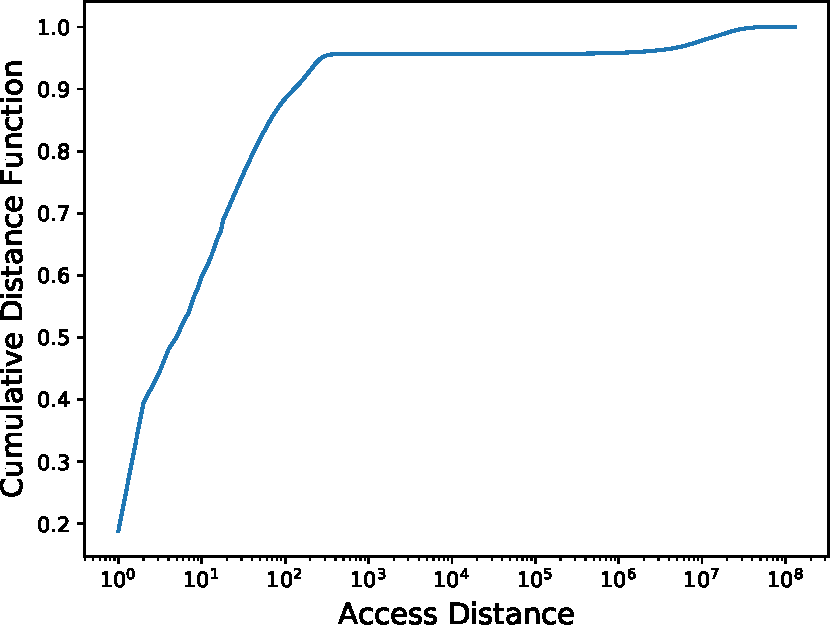
\includegraphics[width=\linewidth]{Q2addtrace1.pdf}
  \caption{Part2: CDF of access distance for prog1.c}
  \label{fig:sub1}
\end{subfigure}%
\hspace{2mm}
\begin{subfigure}{.465\textwidth}
  \centering
  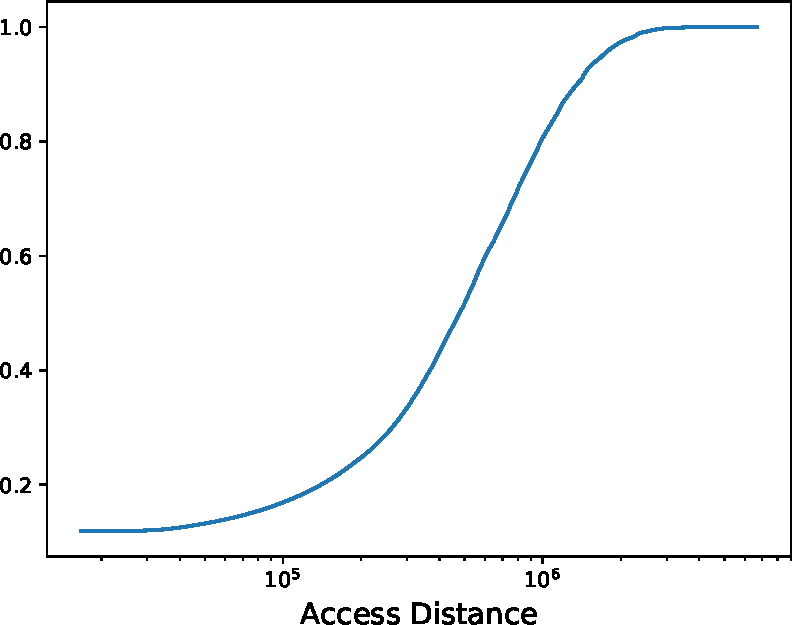
\includegraphics[width=\linewidth]{Q3addtrace1.pdf}
  \caption{Part3: CDF of access distance for misses of prog1.c}
  \label{fig:sub2}
\end{subfigure}
\caption{A comparison between the complete machine access trace and missed machine access trace for \textbf{prog1.c}}
\label{fig:test1}
\vspace{0.8in}
\begin{subfigure}{.48\textwidth}
  \centering
  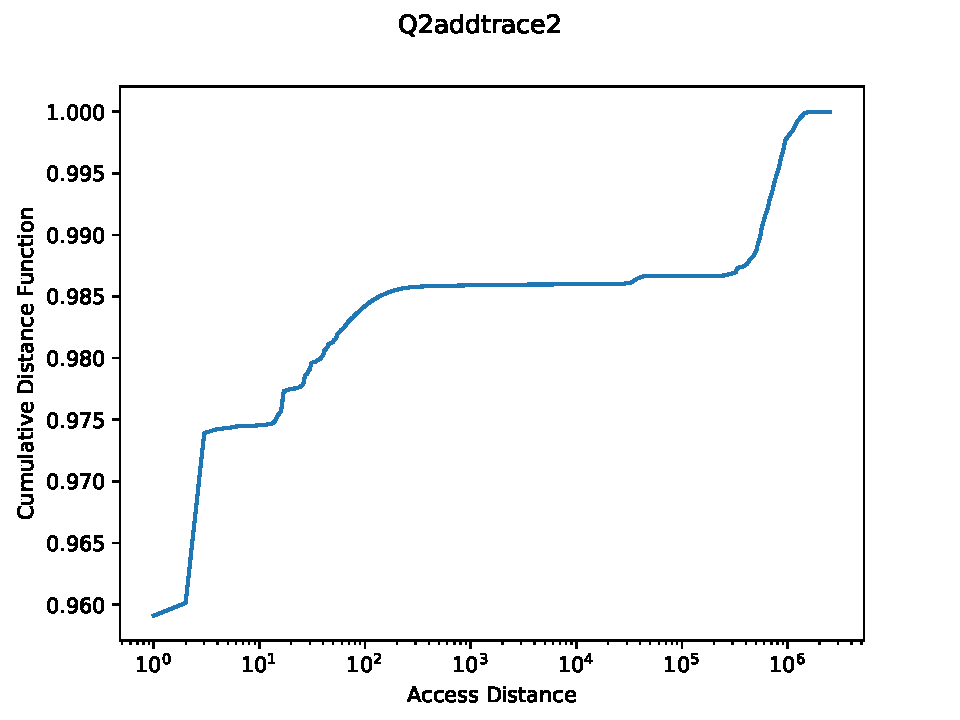
\includegraphics[width=\linewidth]{Q2addtrace2.pdf}
  \caption{Part2: CDF of access distance for prog2.c}
  \label{fig:sub3}
\end{subfigure}%
\hspace{2mm}
\begin{subfigure}{.465\textwidth}
  \centering
  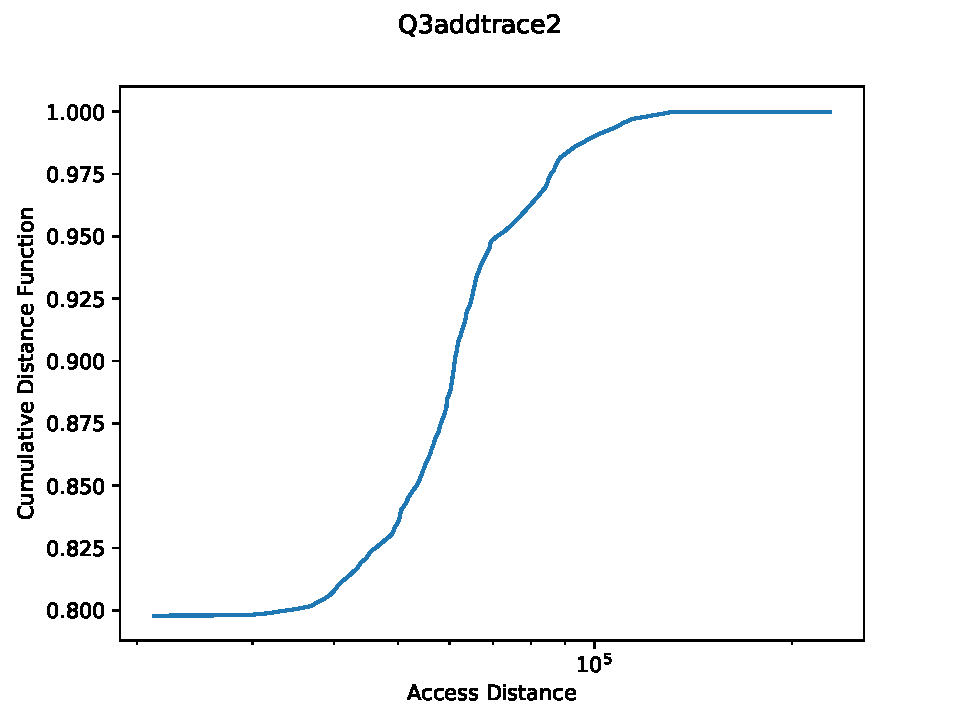
\includegraphics[width=\linewidth]{Q3addtrace2.pdf}
  \caption{Part3: CDF of access distance for misses of prog2.c}
  \label{fig:sub4}
\end{subfigure}
\caption{A comparison between the complete machine access trace and missed machine access trace for \textbf{prog2.c}}
\label{fig:test2}
\end{figure}

% \newpage

\begin{figure}[H]
\centering
\begin{subfigure}{.48\textwidth}
  \centering
  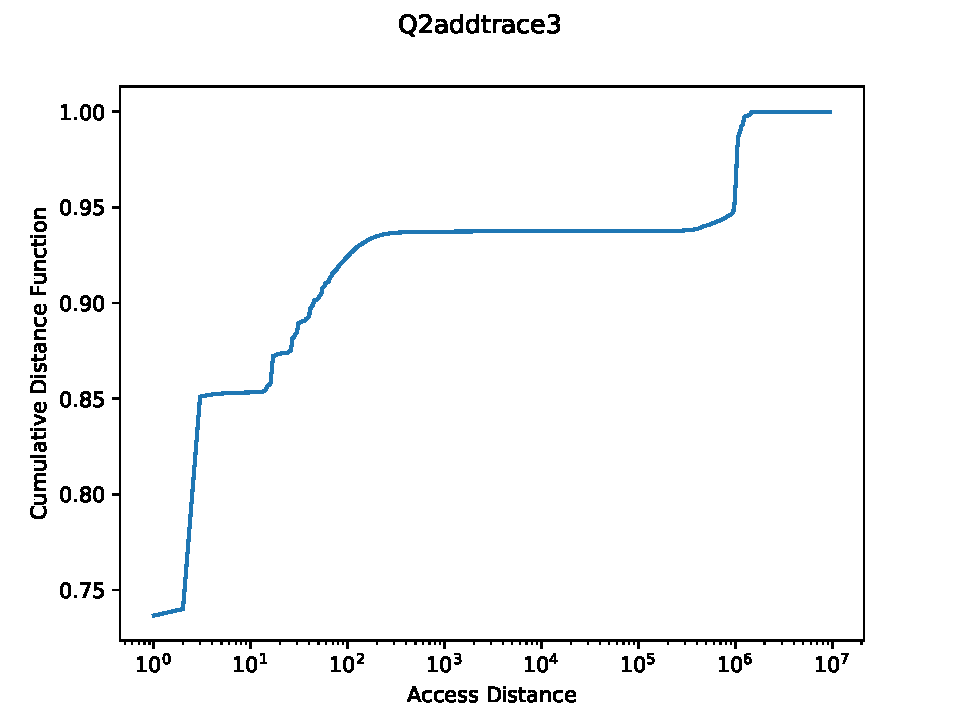
\includegraphics[width=\linewidth]{Q2addtrace3.pdf}
  \caption{Part2: CDF of access distance for prog3.c}
  \label{fig:3sub1}
\end{subfigure}%\hspace{2mm}
\hspace{2mm}
\begin{subfigure}{.465\textwidth}
  \centering
  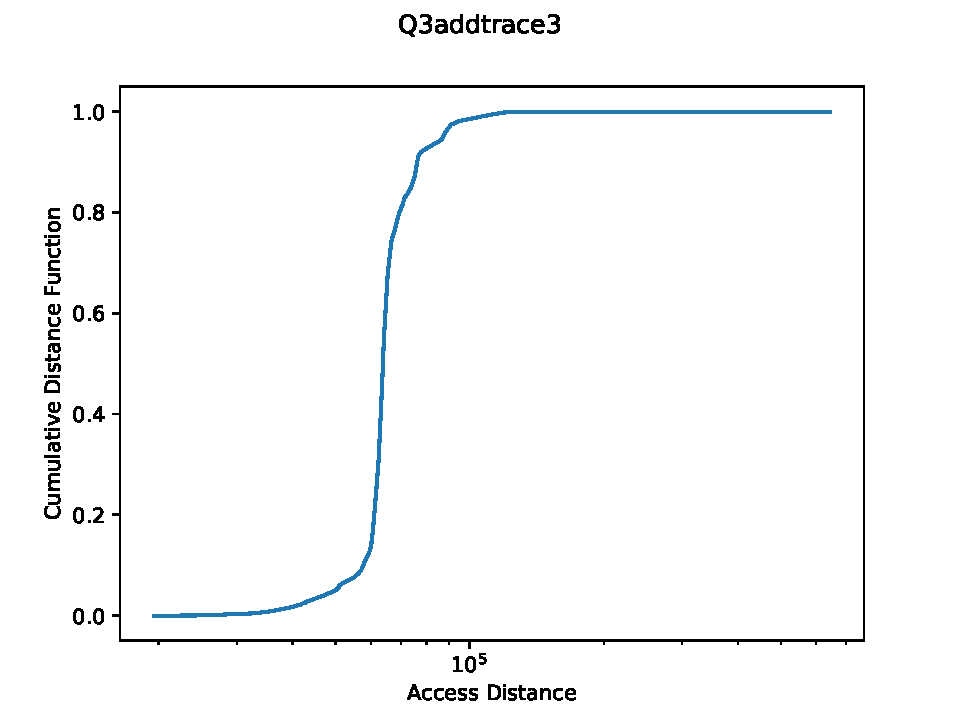
\includegraphics[width=\linewidth]{Q3addtrace3.pdf}
  \caption{Part3: CDF of access distance for misses of prog3.c}
  \label{fig:3sub2}
\end{subfigure}
\caption{A comparison between the complete machine access trace and missed machine access trace for \textbf{prog3.c}}
\label{fig:test3}
\vspace{0.8in}
\begin{subfigure}{.48\textwidth}
  \centering
  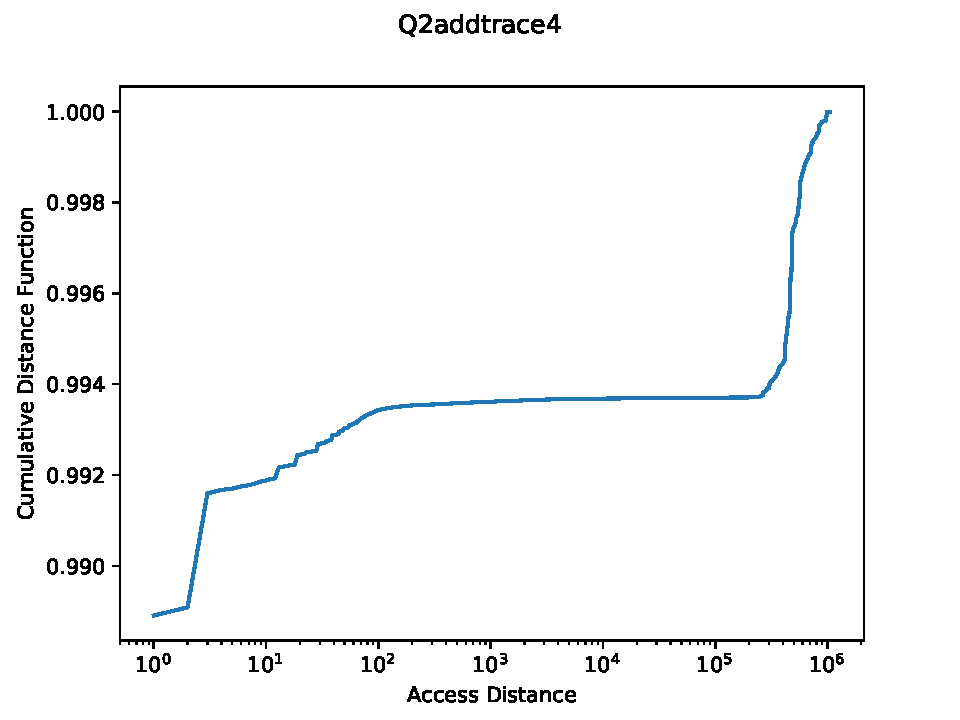
\includegraphics[width=\linewidth]{Q2addtrace4.pdf}
  \caption{Part2: CDF of access distance for prog4.c}
  \label{fig:3sub3}
\end{subfigure}%
\hspace{2mm}
\begin{subfigure}{.465\textwidth}
  \centering
  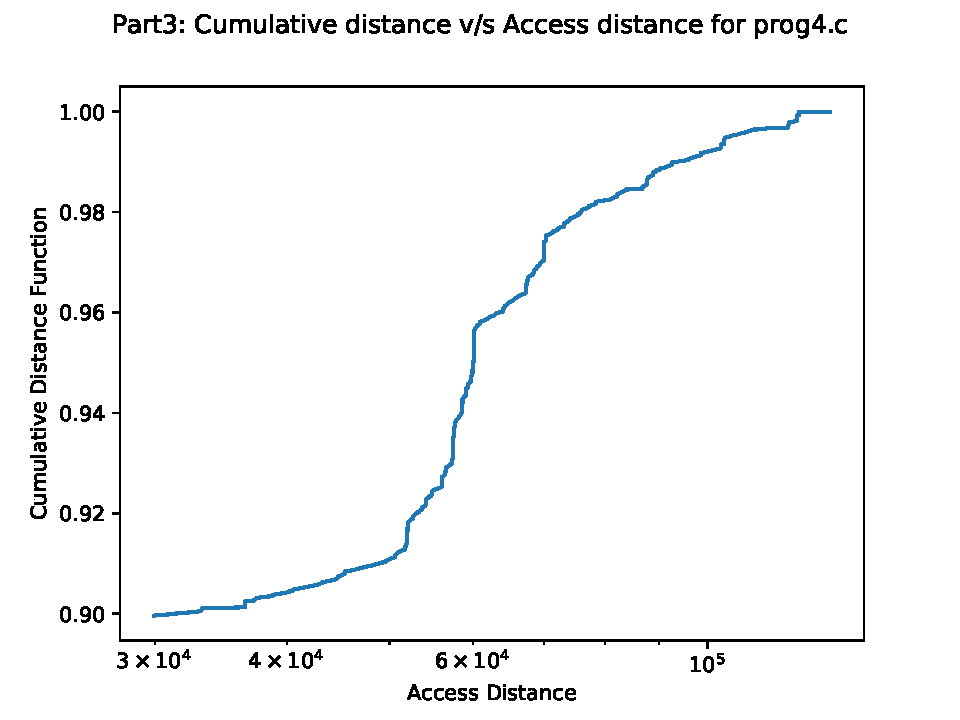
\includegraphics[width=\linewidth]{Q3addtrace4.pdf}
  \caption{Part3: CDF of access distance for misses of prog4.c}
  \label{fig:3sub4}
\end{subfigure}
\caption{A comparison between the complete machine access trace and missed machine access trace for \textbf{prog4.c}}
\label{fig:test4}
\end{figure}


\newpage
\subsection*{PART 3: Hits and Misses}
The cumulative distribution function for part-3 is counted specifically against the misses after
modelling the single-level cache to the obtained traces.
\begin{table}[h]
\centering
\begin{tabular}{ |c|c|c|c|c| } 
\hline
& \textbf{prog1.c} & \textbf{prog2.c} & \textbf{prog3.c} & \textbf{prog4.c} \\
\hline
\textbf{Hits}   & 122297455 & 2295505 & 8862896 & 930888 \\
\hline
\textbf{Misses} & 6690582   & 229068  & 645364  & 130626 \\
\hline
\end{tabular}
\caption{Result of modelling a 2MB 16-Way Cache on the traces}
\end{table}